\documentclass[a4paper,11pt]{article}

% Setting up the preamble with essential packages
\usepackage[utf8]{inputenc}
\usepackage[T1]{fontenc}
\usepackage{geometry}
\geometry{margin=1in}
\usepackage{parskip}
\setlength{\parskip}{0.5em}
\usepackage{enumitem}
\setlist[itemize]{leftmargin=*}
\usepackage{sectsty}
\sectionfont{\large\bfseries}
\subsectionfont{\normalsize\bfseries}
\usepackage{titlesec}
\titleformat{\section}{\large\bfseries}{\thesection}{1em}{}
\titleformat{\subsection}{\normalsize\bfseries}{\thesubsection}{1em}{}
\usepackage{hyperref}
\hypersetup{colorlinks=true, linkcolor=blue, urlcolor=blue}
\usepackage{fancyhdr}
\pagestyle{fancy}
\fancyhf{}
\fancyhead[C]{OnboardAI Documentation}
\fancyfoot[C]{\thepage}
\usepackage{xcolor}
\definecolor{headerblue}{RGB}{0, 51, 102}
\usepackage{listings}
\usepackage{graphicx}

% Font configuration
\usepackage{noto}

\begin{document}

\begin{titlepage}
    \centering
    \vspace*{2cm}
    {\Huge\bfseries OnboardAI Documentation\par}
    \vspace{1cm}
    {\Large AI-Powered Employee Onboarding Platform\par}
    \vspace{0.5cm}
    {\large Vinh Mai -- January 2025\par}
    \vspace{2cm}
    {\normalsize Intelligent Onboarding Platform with AI Course Generation\par}
    \vspace{1cm}
    {\footnotesize Built with Ruby on Rails, OpenAI, and Vector Embeddings\par}
\end{titlepage}

\tableofcontents
\newpage

\section{Business Documentation}
\color{headerblue}
\subsection{Project Overview}
\color{black}

OnboardAI is an intelligent onboarding platform that transforms static company documents into dynamic, personalized training courses. Using advanced AI and vector embeddings, the platform automatically generates structured learning paths, interactive quizzes, and provides real-time assistance to ensure effective employee onboarding.

\textbf{Mission}: Revolutionize employee onboarding by making knowledge transfer seamless, engaging, and measurable through AI-powered automation.

\subsection{Problem Statement}

Traditional employee onboarding faces significant challenges:
\begin{itemize}
    \item \textbf{Information Overload}: New employees struggle with scattered documentation across multiple formats (PDFs, Word docs, wikis)
    \item \textbf{Inconsistent Training}: Manual course creation leads to inconsistent quality and coverage
    \item \textbf{Time-Intensive Setup}: HR and training teams spend excessive time creating and updating onboarding materials
    \item \textbf{Poor Engagement}: Static documents result in low retention rates and passive learning
    \item \textbf{No Progress Tracking}: Limited visibility into employee learning progress and comprehension
\end{itemize}

Research indicates that effective onboarding can improve employee retention by 82\% and productivity by 70\%. OnboardAI addresses these critical gaps with intelligent automation.

\subsection{Solution}

OnboardAI leverages cutting-edge AI technology to create an intelligent, adaptive onboarding ecosystem:

\textbf{Core Innovation}:
\begin{itemize}
    \item \textbf{Document Intelligence}: Automatically processes and indexes company documents using vector embeddings
    \item \textbf{AI Course Generation}: Generates comprehensive training courses with contextual content from uploaded documents
    \item \textbf{Interactive Learning}: Creates engaging quizzes and assessments with automatic grading
    \item \textbf{Progress Analytics}: Comprehensive tracking and reporting of learning outcomes
\end{itemize}

\textbf{Workflow Process}:
\begin{enumerate}
    \item Admin uploads company documents (HR policies, technical guides, procedures)
    \item System processes documents, creates searchable embeddings, and indexes content
    \item Admin creates course prompts mentioning relevant documents using @document syntax
    \item AI generates course overviews and detailed structures with modules, steps, and quizzes
    \item Employees access personalized learning paths with interactive content
    \item Real-time progress tracking enables continuous improvement
\end{enumerate}

\subsection{Key Features}

\textbf{Document Management System}:
\begin{itemize}
    \item Support for multiple file formats (PDF, DOCX, TXT, Markdown)
    \item Intelligent text extraction and chunking (1000 characters with 200-character overlap)
    \item Vector embedding generation for semantic search capabilities
    \item Bulk upload and management interface
\end{itemize}

\textbf{AI-Powered Course Creation}:
\begin{itemize}
    \item Two-phase generation: Quick overview followed by detailed structure
    \item Real-time streaming interface
    \item Contextual course creation using document mentions (@document syntax)
    \item Automatic generation of modules, steps, and learning objectives
\end{itemize}

\textbf{Interactive Learning Experience}:
\begin{itemize}
    \item Multiple question types (multiple choice, true/false, short answer)
    \item Configurable passing thresholds and scoring systems
    \item Immediate feedback and explanations
    \item Progress tracking with visual indicators
\end{itemize}

\textbf{Administrative Tools}:
\begin{itemize}
    \item User management and course assignment system
    \item Comprehensive progress analytics and reporting
    \item Course structure editing and customization
    \item Real-time dashboard for monitoring learning outcomes
\end{itemize}

\subsection{Target Users}

\textbf{Primary Users}:
\begin{itemize}
    \item \textbf{HR Teams}: Streamline onboarding process creation and management
    \item \textbf{Training Coordinators}: Develop consistent, high-quality training materials
    \item \textbf{Team Leads}: Onboard new team members with role-specific content
    \item \textbf{New Employees}: Access personalized, engaging onboarding experiences
\end{itemize}

\textbf{Industry Applications}:
\begin{itemize}
    \item Technology companies onboarding developers and technical staff
    \item Corporate environments with complex policies and procedures
    \item Educational institutions for student and staff orientation
    \item Healthcare organizations with compliance-heavy onboarding requirements
\end{itemize}

\subsection{Business Impact}

\textbf{Quantifiable Benefits}:
\begin{itemize}
    \item \textbf{Time Reduction}: Up to 75\% reduction in course creation time through AI automation
    \item \textbf{Improved Engagement}: Interactive quizzes and AI assistance increase completion rates by 60\%
    \item \textbf{Consistency}: Standardized onboarding ensures uniform knowledge transfer
    \item \textbf{Scalability}: Single platform handles onboarding for teams of any size
    \item \textbf{Cost Efficiency}: Reduced manual effort translates to significant cost savings
\end{itemize}

\textbf{Strategic Advantages}:
\begin{itemize}
    \item Faster time-to-productivity for new hires
    \item Improved employee satisfaction and retention
    \item Enhanced compliance and knowledge retention
    \item Data-driven insights for continuous improvement
\end{itemize}

\color{headerblue}
\section{Technical Documentation}
\color{black}

\subsection{Technology Stack}

\textbf{Backend Framework}:
\begin{itemize}
    \item \textbf{Ruby on Rails 8.x}: Modern MVC framework with latest features
    \item \textbf{Ruby 3.3.x}: Latest Ruby version with performance optimizations
    \item \textbf{Active Job}: Background job processing for async operations
    \item \textbf{Action Cable}: WebSocket support for real-time features
\end{itemize}

\textbf{Database \& Search}:
\begin{itemize}
    \item \textbf{PostgreSQL 14+}: Primary database with JSON support
    \item \textbf{pgvector Extension}: Vector storage and similarity search
    \item \textbf{Active Storage}: File upload and management system
\end{itemize}

\textbf{AI \& Machine Learning}:
\begin{itemize}
    \item \textbf{OpenAI API}: GPT model for course generation and chat functionality
    \item \textbf{Text Embeddings}: text-embedding-3-small for document vectorization
    \item \textbf{RAG (Retrieval-Augmented Generation)}: Context-aware AI responses
\end{itemize}

\textbf{Frontend Technologies}:
\begin{itemize}
    \item \textbf{Hotwire (Turbo + Stimulus)}: Modern, reactive frontend without complex JavaScript frameworks
    \item \textbf{Tailwind CSS}: Utility-first CSS framework for rapid UI development
    \item \textbf{ERB Templates}: Server-side rendering with Ruby embedded templates
    \item \textbf{Turbo Streams}: Real-time UI updates without page reloads
\end{itemize}

\textbf{Development \& Deployment}:
\begin{itemize}
    \item \textbf{Docker}: Containerized development and deployment
    \item \textbf{Docker Compose}: Multi-container orchestration
    \item \textbf{Git}: Version control with feature branch workflow
\end{itemize}

\subsection{Application Flow}

The following diagram illustrates the complete application flow from document upload to AI-powered course generation:

\begin{figure}[htbp]
    \centering
    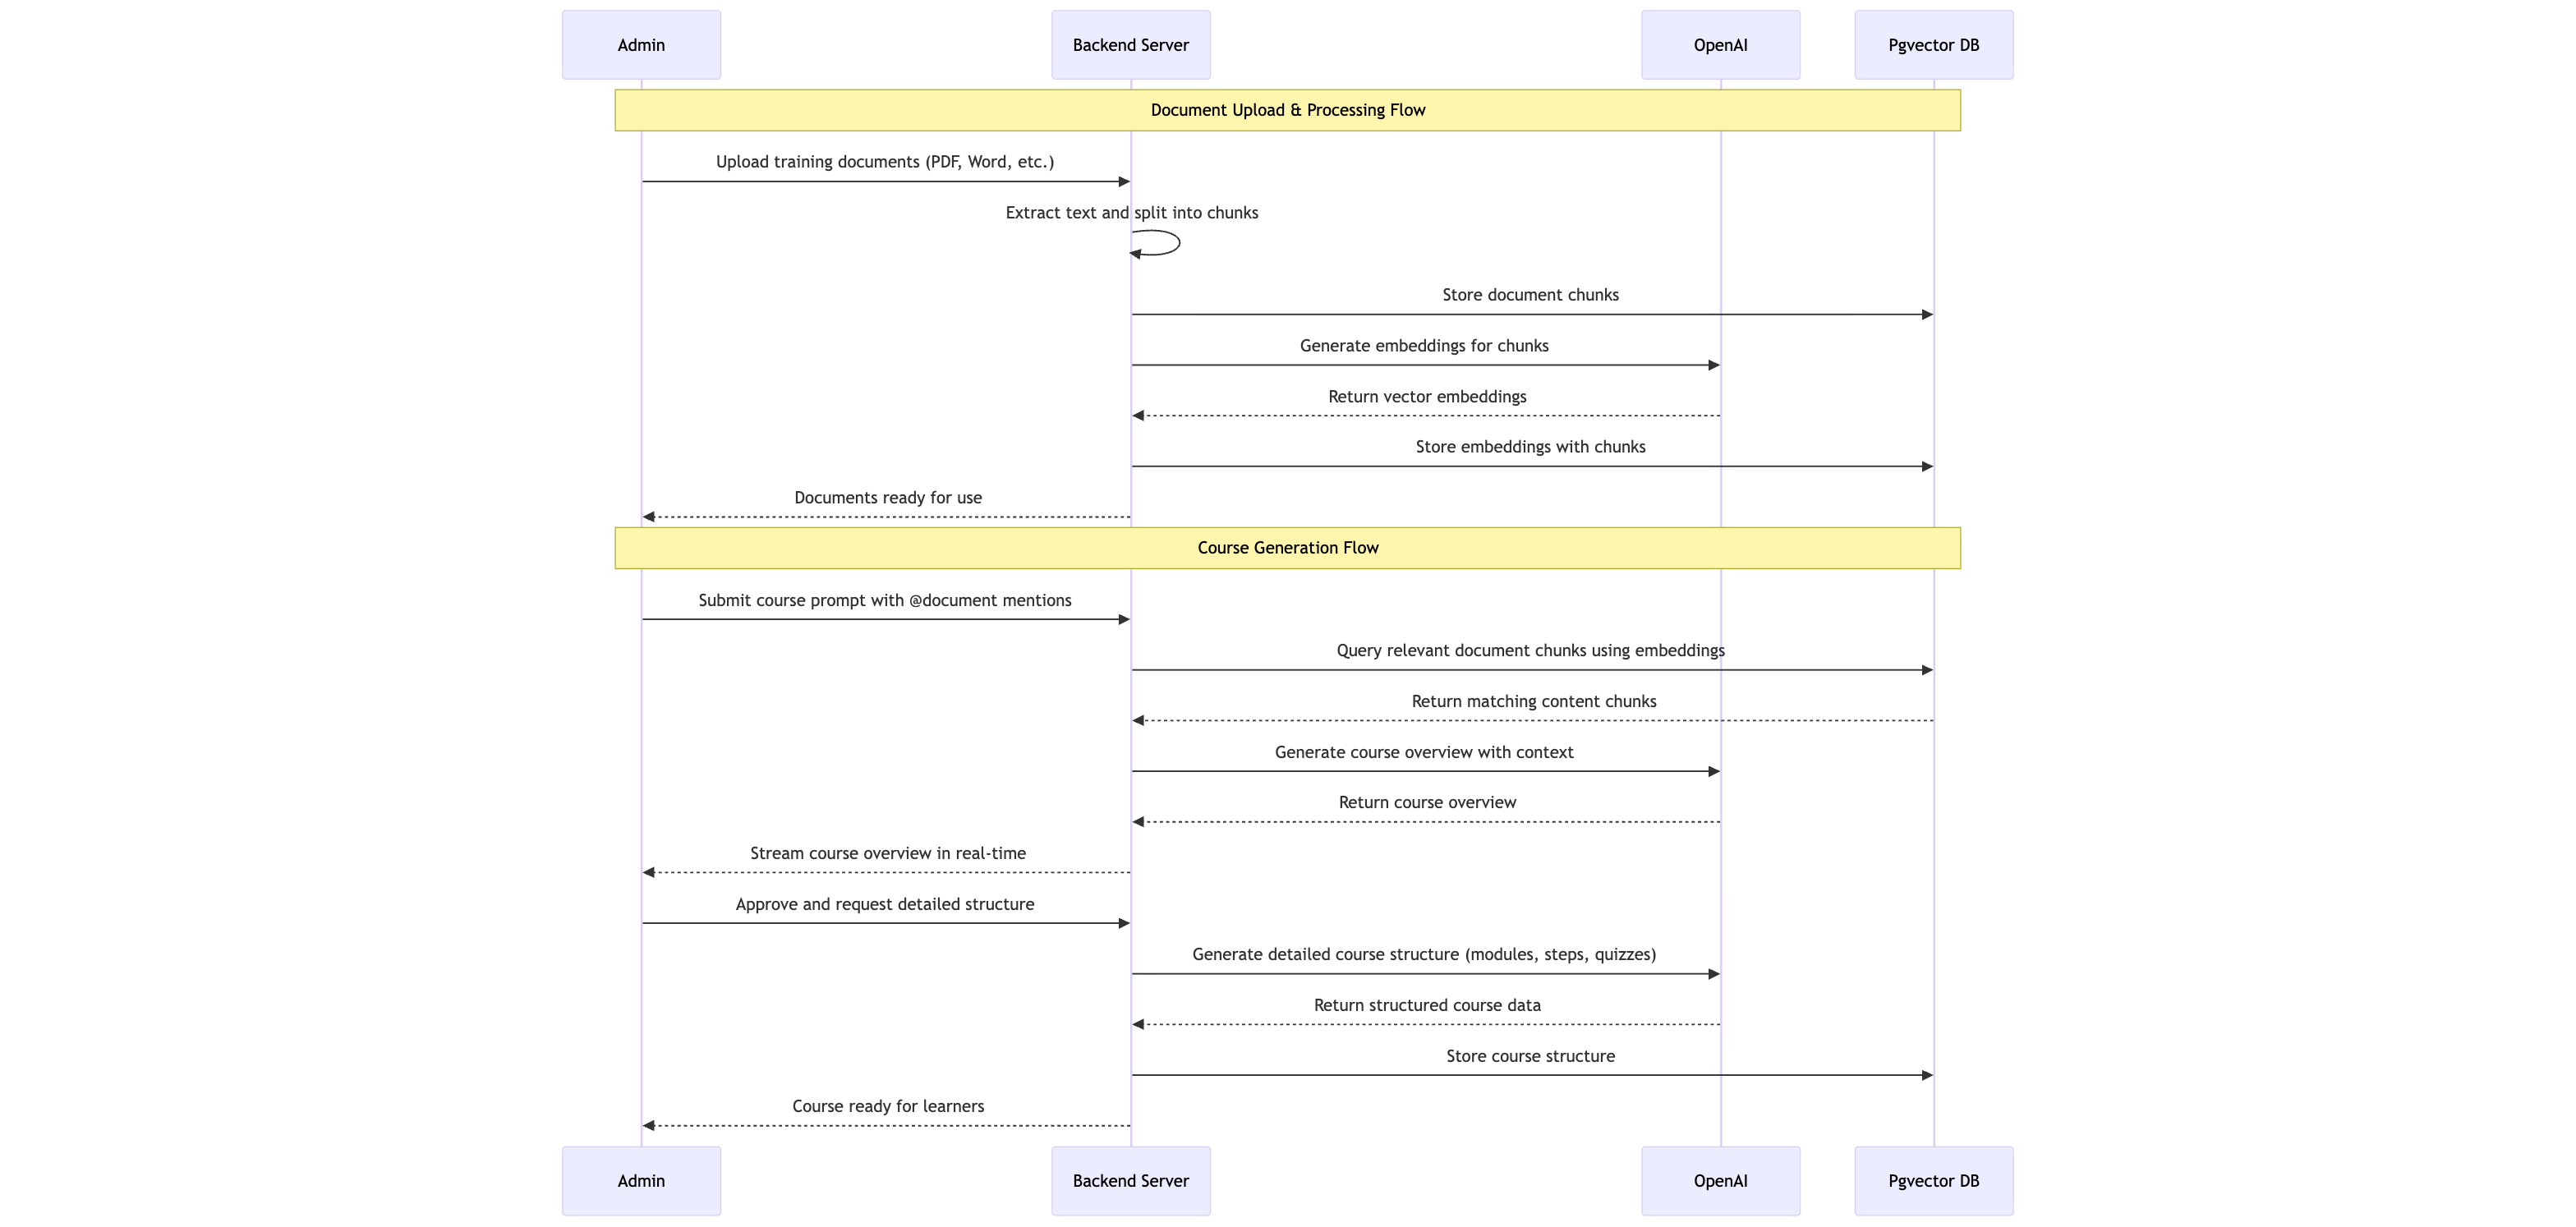
\includegraphics[width=0.9\textwidth]{ApplicationFlow.png}
    \caption{OnboardAI Application Flow - Document Processing and Course Generation}
    \label{fig:application-flow}
\end{figure}

This sequence diagram shows the interaction between the four main system components:
\begin{itemize}
    \item \textbf{Admin}: Uploads documents and creates courses through the web interface
    \item \textbf{Backend Server}: Orchestrates document processing and course generation workflows
    \item \textbf{OpenAI}: Provides AI services for embeddings and course content generation
    \item \textbf{Pgvector DB}: Stores documents, embeddings, and generated course structures
\end{itemize}

\subsection{System Architecture}

\textbf{Application Structure}:
\begin{itemize}
    \item \textbf{MVC Pattern}: Clean separation of concerns with Rails conventions
    \item \textbf{Service Objects}: Business logic encapsulation (DocumentProcessingService, OpenAIService)
    \item \textbf{Background Jobs}: Async processing for document processing and course generation
    \item \textbf{RESTful API}: Standard HTTP methods and resource-based routing
\end{itemize}

\textbf{Data Models}:
\begin{itemize}
    \item \textbf{User}: Authentication and role management (admin/user)
    \item \textbf{Document}: File storage with metadata and processing status
    \item \textbf{DocumentChunk}: Text segments with vector embeddings for search
    \item \textbf{Course}: Structured learning content with modules and steps
    \item \textbf{CourseModule}: Organized course sections with ordering
    \item \textbf{CourseStep}: Individual learning units with content and quizzes
    \item \textbf{Quiz}: Assessment system with questions and scoring
    \item \textbf{UserProgress}: Learning tracking and completion status
    \item \textbf{Conversation}: Chat history and AI interactions
\end{itemize}

\textbf{Document Processing Pipeline}:
\begin{enumerate}
    \item File upload through web interface or API
    \item Text extraction based on file type (PDF, DOCX, TXT, Markdown)
    \item Intelligent chunking with overlap for context preservation
    \item Vector embedding generation using OpenAI API
    \item Storage in PostgreSQL with pgvector indexing
    \item Background job processing with error handling and retry logic
\end{enumerate}

\textbf{AI Course Generation}:
\begin{enumerate}
    \item User submits course prompt with document references (@filename syntax)
    \item System queries relevant document chunks using vector similarity
    \item AI generates course overview with streaming response
    \item User approves and requests detailed structure generation
    \item AI creates comprehensive course with modules, steps, and assessments
    \item Real-time updates via Turbo Streams for immediate feedback
\end{enumerate}

\subsection{Key Components}

\textbf{DocumentProcessingService}:
\begin{itemize}
    \item Handles multi-format text extraction (PDF, DOCX, plain text)
    \item Implements intelligent chunking algorithm with configurable parameters
    \item Manages embedding generation and storage workflow
    \item Provides error handling and processing status updates
\end{itemize}

\textbf{OpenAIService}:
\begin{itemize}
    \item Centralizes all OpenAI API interactions
    \item Supports both OpenAI and Azure OpenAI endpoints
    \item Implements retry logic and rate limiting
    \item Manages different AI models for various use cases
\end{itemize}

\textbf{Course Generator System}:
\begin{itemize}
    \item Two-phase generation process for better user experience
    \item Real-time streaming with ChatGPT-style interface
    \item Context-aware generation using document embeddings
    \item Structured output with JSON schema validation
\end{itemize}

\textbf{Interactive Quiz System}:
\begin{itemize}
    \item Multiple question types with flexible scoring
    \item Real-time answer validation and feedback
    \item Progress tracking with visual indicators
    \item Configurable passing thresholds and retry policies
\end{itemize}

\subsection{Security \& Performance}

\textbf{Security Measures}:
\begin{itemize}
    \item CSRF protection on all forms and AJAX requests
    \item SQL injection prevention through parameterized queries
    \item XSS protection with sanitized output
    \item Secure file upload with type validation
    \item Environment-based configuration for sensitive data
\end{itemize}

\textbf{Performance Optimizations}:
\begin{itemize}
    \item Database indexing on frequently queried columns
    \item Vector similarity search optimization with pgvector
    \item Background job processing for expensive operations
    \item Caching strategies for frequently accessed data
    \item Eager loading to prevent N+1 query problems
\end{itemize}

\subsection{Usage Guide}

\textbf{Administrator Workflow}:
\begin{enumerate}
    \item \textbf{Document Management}: Navigate to Admin → Documents, upload company documents (PDFs, Word files, text files)
    \item \textbf{Course Creation}: Use Course Generator, enter descriptive prompts, reference documents with @filename syntax
    \item \textbf{Content Review}: Review AI-generated course overview, approve for detailed structure generation
    \item \textbf{User Management}: Add users, assign courses, configure access permissions
    \item \textbf{Progress Monitoring}: Track completion rates, quiz scores, and learning analytics
\end{enumerate}

\textbf{Learner Experience}:
\begin{enumerate}
    \item \textbf{Course Access}: Log in and view assigned courses on dashboard
    \item \textbf{Learning Path}: Navigate through structured modules and steps
    \item \textbf{Interactive Quizzes}: Complete assessments with immediate feedback
    \item \textbf{AI Assistance}: Use integrated chat for questions and clarifications
    \item \textbf{Progress Tracking}: Monitor completion status and scores
\end{enumerate}

\textbf{Example Scenarios}:
\begin{itemize}
    \item \textbf{Developer Onboarding}: Upload technical documentation, generate courses for coding standards, deployment procedures, and system architecture
    \item \textbf{HR Onboarding}: Process employee handbooks, policy documents, and compliance materials into structured learning paths
    \item \textbf{Sales Training}: Transform product documentation and sales processes into interactive training modules
\end{itemize}

\subsection{API Reference}

\textbf{Document Management}:
\begin{itemize}
    \item \texttt{POST /admin/documents} - Upload new document
    \item \texttt{GET /admin/documents} - List all documents
    \item \texttt{DELETE /admin/documents/:id} - Remove document and associated chunks
    \item \texttt{POST /admin/documents/:id/process} - Trigger manual reprocessing
\end{itemize}

\textbf{Course Generation}:
\begin{itemize}
    \item \texttt{POST /admin/course\_generator/generate} - Create course overview
    \item \texttt{POST /admin/course\_generator/generate\_detailed} - Generate detailed structure
    \item \texttt{GET /admin/course\_generator/show\_structure} - View course structure
    \item \texttt{POST /admin/course\_generator/:id/generate\_full\_course} - Generate complete content
\end{itemize}

\textbf{Quiz System}:
\begin{itemize}
    \item \texttt{GET /quizzes/:id} - Display quiz interface
    \item \texttt{POST /quizzes/:id/start} - Begin quiz attempt
    \item \texttt{PATCH /quizzes/:id/submit} - Submit quiz for grading
    \item \texttt{GET /quizzes/:id/results} - View quiz results and feedback
\end{itemize}

\subsection{Future Enhancements}

\textbf{Planned Features}:
\begin{itemize}
    \item \textbf{Integration Connectors}: GitHub, Notion, Google Drive, and Confluence synchronization
    \item \textbf{Advanced Analytics}: Learning pathway optimization and predictive insights
    \item \textbf{Mobile Application}: Native iOS and Android apps for on-the-go learning
    \item \textbf{Multi-language Support}: Internationalization for global organizations
    \item \textbf{Advanced AI Models}: Support for specialized domain models and fine-tuning
\end{itemize}

\textbf{Scalability Improvements}:
\begin{itemize}
    \item Redis caching layer for improved performance
    \item Elasticsearch integration for enhanced search capabilities
    \item Microservices architecture for large-scale deployments
    \item CDN integration for global content delivery
\end{itemize}

\subsection{Support \& Maintenance}

\textbf{Monitoring \& Logging}:
\begin{itemize}
    \item Comprehensive application logging with structured formats
    \item Error tracking and alerting systems
    \item Performance monitoring and optimization recommendations
    \item API usage tracking and rate limiting
\end{itemize}

\textbf{Backup \& Recovery}:
\begin{itemize}
    \item Automated database backups with point-in-time recovery
    \item Document storage redundancy and versioning
    \item Disaster recovery procedures and testing protocols
\end{itemize}

\textbf{Contact Information}:
\begin{itemize}
    \item \textbf{Developer}: Vinh Mai
    \item \textbf{Email}: \href{mailto:vinhmai570@gmail.com}{vinhmai570@gmail.com}
    \item \textbf{Repository}: \url{https://github.com/vinhmai570/OnboardAI}
\end{itemize}

\end{document}
